\documentclass[11pt,compress,t,notes=noshow, xcolor=table]{beamer}
\usepackage[]{graphicx}\usepackage[]{color}
% maxwidth is the original width if it is less than linewidth
% otherwise use linewidth (to make sure the graphics do not exceed the margin)
\makeatletter
\def\maxwidth{ %
  \ifdim\Gin@nat@width>\linewidth
    \linewidth
  \else
    \Gin@nat@width
  \fi
}
\makeatother

\definecolor{fgcolor}{rgb}{0.345, 0.345, 0.345}
\newcommand{\hlnum}[1]{\textcolor[rgb]{0.686,0.059,0.569}{#1}}%
\newcommand{\hlstr}[1]{\textcolor[rgb]{0.192,0.494,0.8}{#1}}%
\newcommand{\hlcom}[1]{\textcolor[rgb]{0.678,0.584,0.686}{\textit{#1}}}%
\newcommand{\hlopt}[1]{\textcolor[rgb]{0,0,0}{#1}}%
\newcommand{\hlstd}[1]{\textcolor[rgb]{0.345,0.345,0.345}{#1}}%
\newcommand{\hlkwa}[1]{\textcolor[rgb]{0.161,0.373,0.58}{\textbf{#1}}}%
\newcommand{\hlkwb}[1]{\textcolor[rgb]{0.69,0.353,0.396}{#1}}%
\newcommand{\hlkwc}[1]{\textcolor[rgb]{0.333,0.667,0.333}{#1}}%
\newcommand{\hlkwd}[1]{\textcolor[rgb]{0.737,0.353,0.396}{\textbf{#1}}}%
\let\hlipl\hlkwb

\usepackage{framed}
\makeatletter
\newenvironment{kframe}{%
 \def\at@end@of@kframe{}%
 \ifinner\ifhmode%
  \def\at@end@of@kframe{\end{minipage}}%
  \begin{minipage}{\columnwidth}%
 \fi\fi%
 \def\FrameCommand##1{\hskip\@totalleftmargin \hskip-\fboxsep
 \colorbox{shadecolor}{##1}\hskip-\fboxsep
     % There is no \\@totalrightmargin, so:
     \hskip-\linewidth \hskip-\@totalleftmargin \hskip\columnwidth}%
 \MakeFramed {\advance\hsize-\width
   \@totalleftmargin\z@ \linewidth\hsize
   \@setminipage}}%
 {\par\unskip\endMakeFramed%
 \at@end@of@kframe}
\makeatother

\definecolor{shadecolor}{rgb}{.97, .97, .97}
\definecolor{messagecolor}{rgb}{0, 0, 0}
\definecolor{warningcolor}{rgb}{1, 0, 1}
\definecolor{errorcolor}{rgb}{1, 0, 0}
\newenvironment{knitrout}{}{} % an empty environment to be redefined in TeX

\usepackage{alltt}
\newcommand{\SweaveOpts}[1]{}  % do not interfere with LaTeX
\newcommand{\SweaveInput}[1]{} % because they are not real TeX commands
\newcommand{\Sexpr}[1]{}       % will only be parsed by R
\newcommand{\xmark}{\ding{55}}%


\usepackage[english]{babel}
\usepackage[utf8]{inputenc}

\usepackage{dsfont}
\usepackage{verbatim}
\usepackage{amsmath}
\usepackage{amsfonts}
\usepackage{amssymb}
\usepackage{bm}
\usepackage{csquotes}
\usepackage{multirow}
\usepackage{longtable}
\usepackage{booktabs}
\usepackage{enumerate}
\usepackage[absolute,overlay]{textpos}
\usepackage{psfrag}
\usepackage{algorithm}
\usepackage{algpseudocode}
\usepackage{eqnarray}
\usepackage{arydshln}
\usepackage{tabularx}
\usepackage{placeins}
\usepackage{tikz}
\usepackage{setspace}
\usepackage{colortbl}
\usepackage{mathtools}
\usepackage{wrapfig}
\usepackage{bm}
\usepackage{amsmath}
\usepackage{pifont}
\usepackage{xcolor} %colored math symbols

\usetikzlibrary{shapes,arrows,automata,positioning,calc,chains,trees, shadows}
\tikzset{
  %Define standard arrow tip
  >=stealth',
  %Define style for boxes
  punkt/.style={
    rectangle,
    rounded corners,
    draw=black, very thick,
    text width=6.5em,
    minimum height=2em,
    text centered},
  % Define arrow style
  pil/.style={
    ->,
    thick,
    shorten <=2pt,
    shorten >=2pt,}
}

\usepackage{subfig}

% Defines macros and environments
\usepackage{../../style/lmu-lecture}


\let\code=\texttt
\let\proglang=\textsf

\setkeys{Gin}{width=0.9\textwidth}

\setbeamertemplate{frametitle}{\expandafter\uppercase\expandafter\insertframetitle}

\usepackage{bbm}
% basic latex stuff
\newcommand{\pkg}[1]{{\fontseries{b}\selectfont #1}} %fontstyle for R packages
\newcommand{\lz}{\vspace{0.5cm}} %vertical space
\newcommand{\dlz}{\vspace{1cm}} %double vertical space
\newcommand{\oneliner}[1] % Oneliner for important statements
{\begin{block}{}\begin{center}\begin{Large}#1\end{Large}\end{center}\end{block}}


%new environments
\newenvironment{vbframe}  %frame with breaks and verbatim
{
 \begin{frame}[containsverbatim,allowframebreaks]
}
{
\end{frame}
}

\newenvironment{vframe}  %frame with verbatim without breaks (to avoid numbering one slided frames)
{
 \begin{frame}[containsverbatim]
}
{
\end{frame}
}

\newenvironment{blocki}[1]   % itemize block
{
 \begin{block}{#1}\begin{itemize}
}
{
\end{itemize}\end{block}
}

\newenvironment{fragileframe}[2]{  %fragile frame with framebreaks
\begin{frame}[allowframebreaks, fragile, environment = fragileframe]
\frametitle{#1}
#2}
{\end{frame}}


\newcommand{\myframe}[2]{  %short for frame with framebreaks
\begin{frame}[allowframebreaks]
\frametitle{#1}
#2
\end{frame}}

\newcommand{\remark}[1]{
  \textbf{Remark:} #1
}


\newenvironment{deleteframe}
{
\begingroup
\usebackgroundtemplate{
\includegraphics[width=\paperwidth,height=\paperheight]{../style/color/red.png}}
 \begin{frame}
}
{
\end{frame}
\endgroup
}
\newenvironment{simplifyframe}
{
\begingroup
\usebackgroundtemplate{
\includegraphics[width=\paperwidth,height=\paperheight]{../style/color/yellow.png}}
 \begin{frame}
}
{
\end{frame}
\endgroup
}\newenvironment{draftframe}
{
\begingroup
\usebackgroundtemplate{
\includegraphics[width=\paperwidth,height=\paperheight]{../style/color/green.jpg}}
 \begin{frame}
}
{
\end{frame}
\endgroup
}
% https://tex.stackexchange.com/a/261480: textcolor that works in mathmode
\makeatletter
\renewcommand*{\@textcolor}[3]{%
  \protect\leavevmode
  \begingroup
    \color#1{#2}#3%
  \endgroup
}
\makeatother


\input{../../latex-math/basic-math}
\input{../../latex-math/basic-ml}
\input{../../latex-math/ml-nn}

\begin{document}

\lecturechapter{CNN: Conv2D}
\lecture{I2DL}
%%%%%%%%%%%%%%%%%%%%%%%%%%%%%%%%%%%%%%%%%%%%%%%%%%%%%%%%%%%%%%%%%%

\begin{vbframe}{Filters to extract features}
    \begin{itemize}
        \item Filters are widely applied in Computer Vision (CV) since the 70's.
        \item One prominent example: \textbf{Sobel-Filter}.
        \item Detects edges in images.
    \end{itemize}
    \begin{figure}
        \centering
        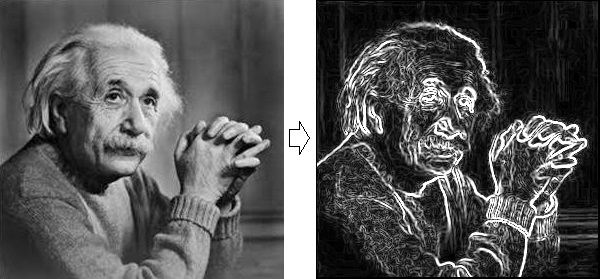
\includegraphics[width=10cm]{figure/sobel_einstein.png}
        % source: https://github.com/qmegas/sobel-operator/blob/HEAD/images/1.jpg
        \caption{Sobel-filtered image.}
    \end{figure}
\framebreak
%%%%%%%%%%%%%%%%%%%%%%%%%%%%%%%%%%%%%%%%%%%%%%%%%%%%%%%%%%%%%%%%%%

\begin{itemize}
\item Edges occur where the intensity over neighboring pixels changes fast.
\item Thus, approximate the gradient of the intensity of each pixel.
\item Sobel showed that the gradient image $\textbf{G}_x$ of original image $\textbf{A}$ in x-dimension  can be approximated by:
$$ \textbf{G}_x = 
\begin{bmatrix}
-1 & 0 & +1 \\
-2 & 0 & +2 \\
-1 & 0 & +1 
\end{bmatrix} * \textbf{A} = \textbf{S}_x * \textbf{A}
$$
where $*$ indicates a mathematical operation known as a \textbf{convolution}, not a traditional matrix multiplication.
\item The filter matrix $\textbf{S}_x$ consists of the product of an \textbf{averaging} and a \textbf{differentiation} kernel: 
$$
\underbrace{\begin{bmatrix}
1 & 2 & 1   
\end{bmatrix}^{T}}_{averaging}
\underbrace{\begin{bmatrix}
-1 & 0 & +1   
\end{bmatrix}}_{differentiation}
$$
\end{itemize}
\framebreak
%%%%%%%%%%%%%%%%%%%%%%%%%%%%%%%%%%%%%%%%%%%%%%%%%%%%%%%%%%%%%%%%%%
    \begin{itemize}
        \item Similarly, the gradient image $\textbf{G}_y$ in y-dimension can be approximated by:
        $$
            \textbf{G}_y = 
            \begin{bmatrix}
                -1 & -2 & -1  \\
                0 & 0 & 0 \\
                +1 & +2 & +1
            \end{bmatrix} * \textbf{A} = \textbf{S}_y * \textbf{A}
        $$
        \item The combination of both gradient images yields a dimension-independent gradient information $\textbf{G}$:
        $$
            \textbf{G} = \sqrt{\textbf{G}_x^2 + \textbf{G}_y^2}
        $$
        \item These matrix operations were used to create the filtered picture of Albert Einstein.
    \end{itemize}
\end{vbframe}
%%%%%%%%%%%%%%%%%%%%%%%%%%%%%%%%%%%%%%%%%%%%%%%%%%%%%%%%%%%%%%%%%%

\begin{frame}{Horizontal vs Vertical edges}
    \begin{figure}
        \centering
          \scalebox{0.9}{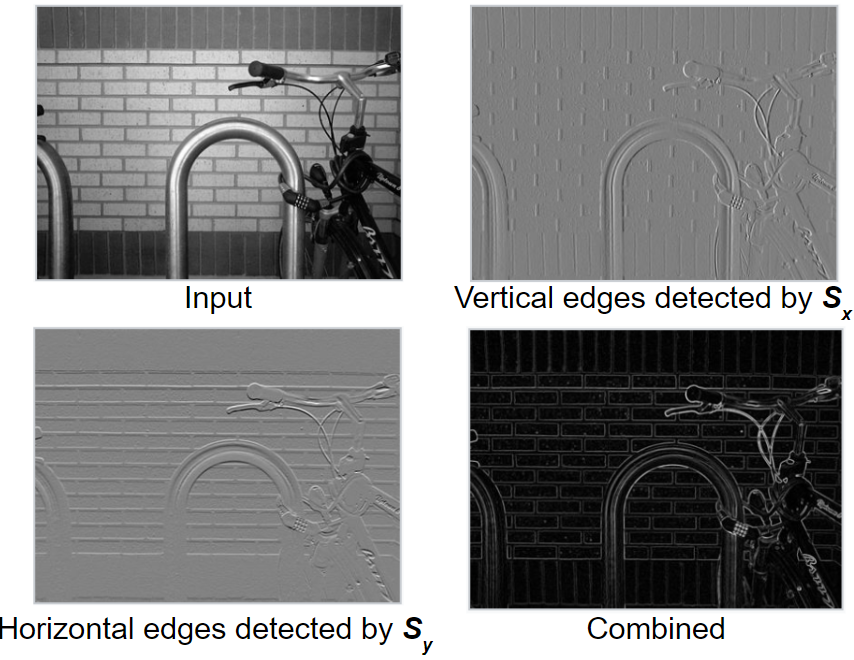
\includegraphics{figure/sobel_bike.png}}
          \tiny{\\ Source: Wikipedia}
         \caption{\footnotesize{Sobel filtered images. Outputs are normalized in each case. }}
    \end{figure}
\end{frame}
%%%%%%%%%%%%%%%%%%%%%%%%%%%%%%%%%%%%%%%%%%%%%%%%%%%%%%%%%%%%%%%%%%

\begin{frame}{Filters to extract features}

    \center
    \only<1>{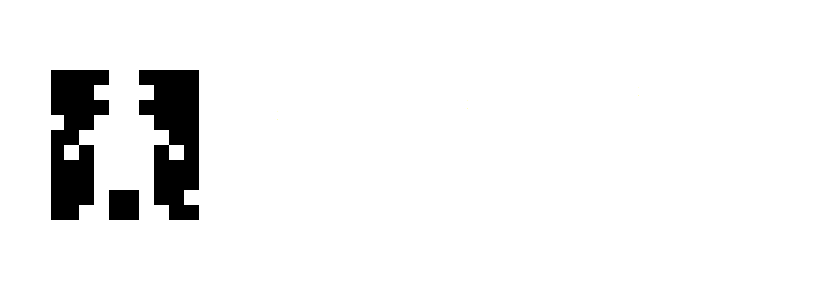
\includegraphics[width=11cm]{figure/sobel1.png}}%
    \only<2>{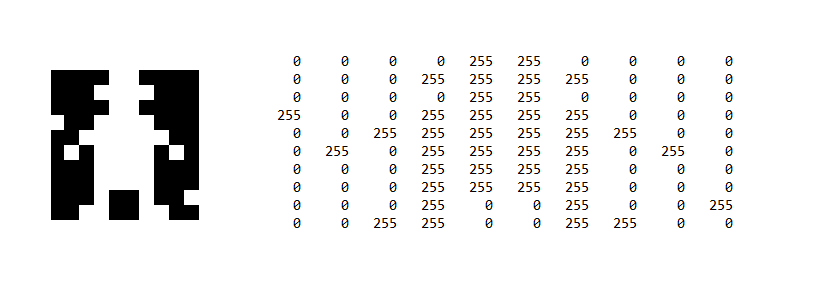
\includegraphics[width=11cm]{figure/sobel2.png}}%
    \only<3>{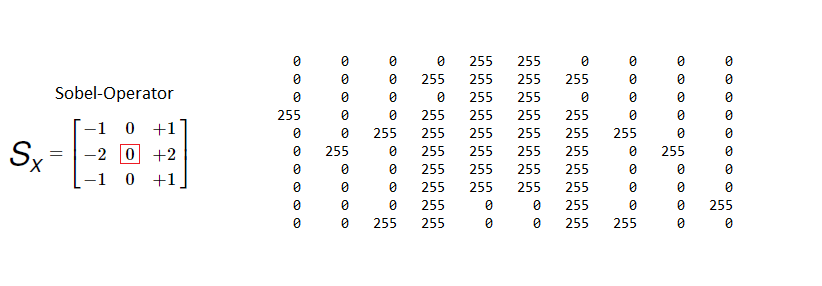
\includegraphics[width=11cm]{figure/sobel3.png}}%
    \only<4>{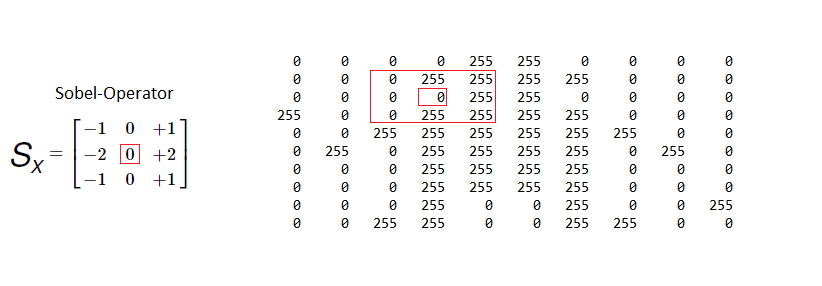
\includegraphics[width=11cm]{figure/sobel4.png}}%
    \only<5>{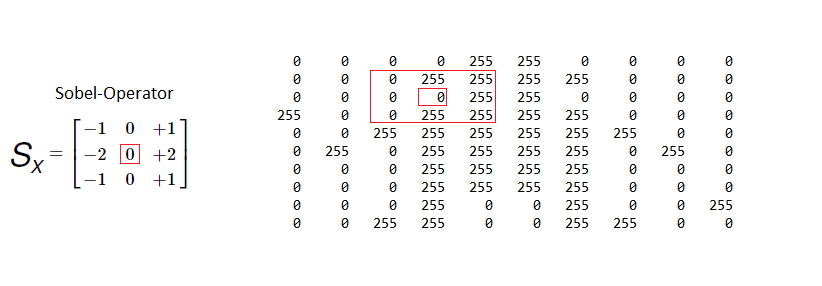
\includegraphics[width=11cm]{figure/sobel4.png}}%
    \only<6>{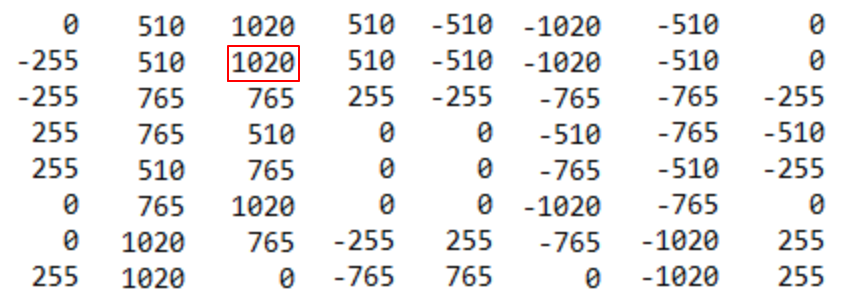
\includegraphics[width=6cm]{figure/sobel6.png}}%
    \only<7>{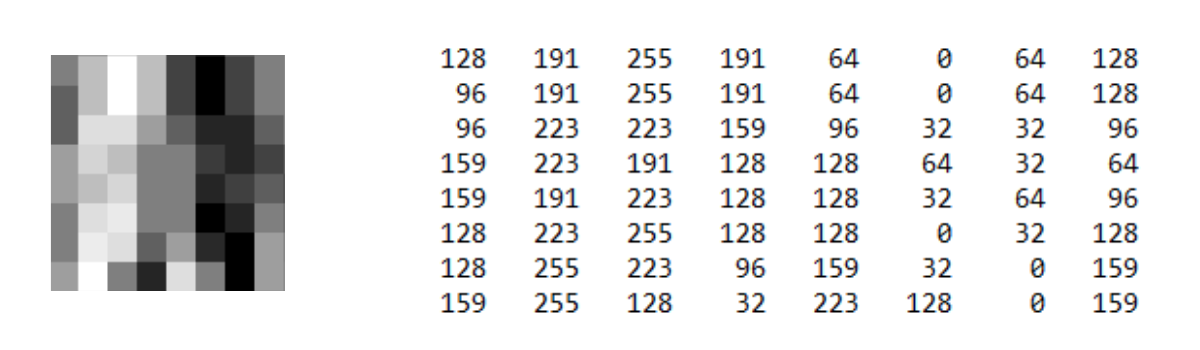
\includegraphics[width=11cm]{figure/sobel8.png}}%

    \begin{itemize}
        \only<1>{\item Let's do this on a dummy image.}
        \only<1>{\item How to represent a digital image?}
        \only<2>{\item Basically as an array of integers.}
        \only<3>{\item $\textbf{S}_x$ enables us to to detect vertical edges!}
        \only<4>{\item[]}
        \only<5>{\item[]
        \vspace{-0.8cm}
        \begin{alignat*}{3}
            (\textbf{G}_x)_{(i,j)} = (\textbf{I} \star \textbf{S}_x)_{(i, j)}
                 & = -1 \cdot 0 \ \ &&+ \ \ 0 \cdot 255 \ \ &&+ \ \ \textbf{1} \cdot \textbf{255} \\
                 &\quad - 2 \cdot 0 &&+ \ \ 0 \cdot 0 &&+ \ \ \textbf{2} \cdot \textbf{255} \\
                 &\quad - 1 \cdot 0 &&+ \ \ 0 \cdot 255 &&+ \ \ \textbf{1} \cdot \textbf{255}
                 \notag
        \end{alignat*}
        }

\only<6>{\item Applying the Sobel-Operator to every location in the input yields us the \textbf{feature map}.}
\only<7>{\item Normalized feature map reveals vertical edges.
\item Note the dimensional reduction compared to the dummy image.}
\end{itemize}
\end{frame}

%%%%%%%%%%%%%%%%%%%%%%%%%%%%%%%%%%%%%%%%%%%%%%%%%%%%%%%%%%%%%%%%%%
\begin{vbframe}{Why do we need to know all of that?}
  \begin{itemize}
    \item What we just did was extracting \textbf{pre-defined} features from our input (i.e. edges).
    \item A convolutional neural network does almost exactly the same: \enquote{extracting features from the input}.
    \item[] $\Rightarrow$ The main difference is that we usually do not tell the CNN what to look for (pre-define them), \textbf{the CNN decides itself}.
    \item In a nutshell:
    \begin{itemize}
      \item We initialize a lot of random filters (like the Sobel but just random entries) and apply them to our input.
      \item Then, a classifier which is generally a feed forward neural net, uses them as input data.
      \item Filter entries will be adjusted by common gradient descent methods.
    \end{itemize}
  \end{itemize}
\end{vbframe}
%%%%%%%%%%%%%%%%%%%%%%%%%%%%%%%%%%%%%%%%%%%%%%%%%%%%%%%%%%%%%%%%%%

\begin{frame}{Why do we need to know all of that?}
\center
\only<1>{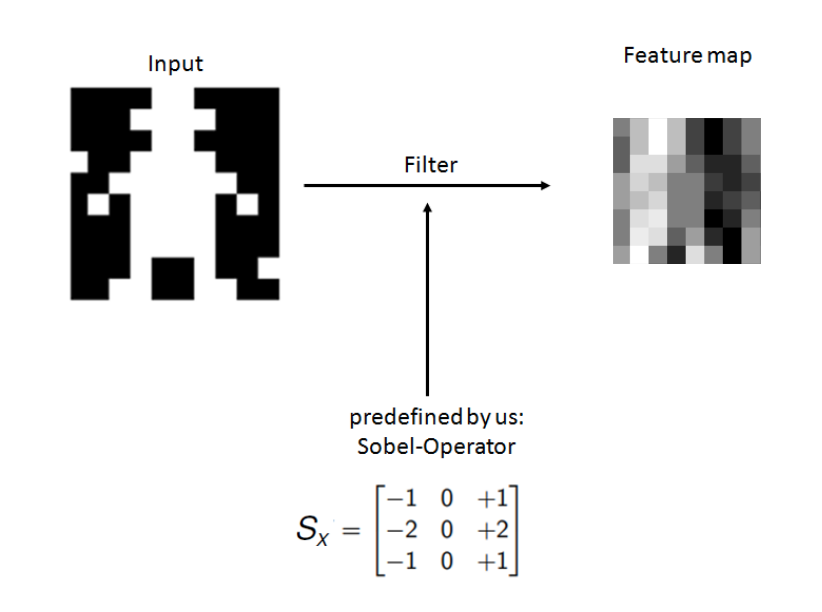
\includegraphics[width=11cm]{figure/sobel9.png}}
\only<2>{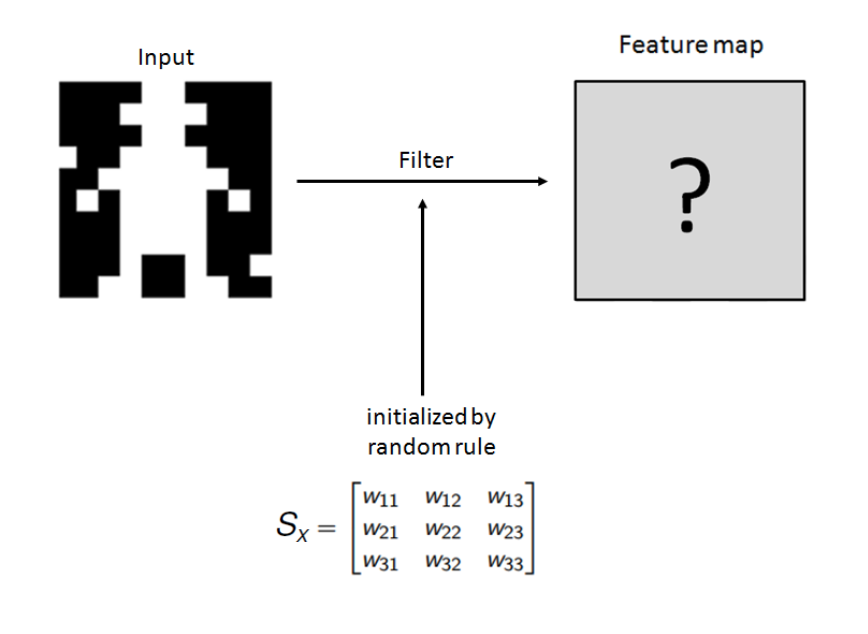
\includegraphics[width=10.5cm]{figure/sobel10.png}}
\end{frame}

%%%%%%%%%%%%%%%%%%%%%%%%%%%%%%%%%%%%%%%%%%%%%%%%%%%%%%%%%%%%%%%%%%
\begin{frame}{Working with images}
  \begin{itemize}
  \item In order to understand the functionality of CNNs, we have to familiarize ourselves with some properties of images.
  \item Grey scale images:
  \begin{itemize}
    \item Matrix with dimensions \textbf{h}eight $\times$ \textbf{w}idth $\times$ 1.
    \item Pixel entries differ from 0 (black) to 255 (white).
  \end{itemize}
  \item Color images:
  \begin{itemize}
    \item Tensor with dimensions \textbf{h}eight $\times$ \textbf{w}idth $\times$ 3.
    \item The depth 3 denotes the RGB values (red - green - blue).
  \end{itemize}
  \item Filters:
  \begin{itemize}
    \item A filter's depth is \textbf{always} equal to the input's depth!
    \item In practice, filters are usually square.
    \item Thus we only need one integer to define its size.
    \item For example, a filter of size $2$ applied on a color image actually has the dimensions $2 \times 2 \times 3$.
  \end{itemize}
  \end{itemize}
\end{frame}
%%%%%%%%%%%%%%%%%%%%%%%%%%%%%%%%%%%%%%%%%%%%%%%%%%%%%%%%%%%%%%%%%%

\begin{frame}{The 2d convolution}
\begin{itemize}
\only<1-8>{\item Suppose we have an input with entries $a, b, \dots, i$ (think of pixel values).}
\only<1-8>{\item The filter we would like to apply has weights $w_{11}, w_{12}, w_{21} \text{ and } w_{22}$.}
\end{itemize}
\center
\only<1>{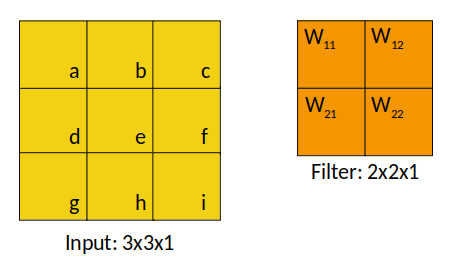
\includegraphics[width=7cm]{figure/conv2d_1.png}}%
\only<2>{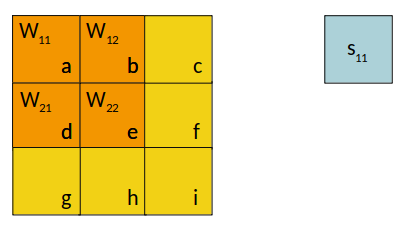
\includegraphics[width=6cm]{figure/conv2d_2.png}}%
\only<3>{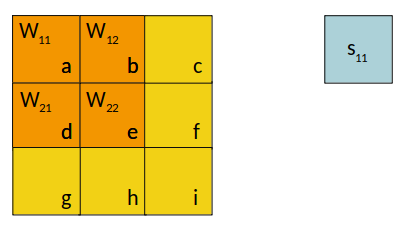
\includegraphics[width=6cm]{figure/conv2d_2.png}}%
\only<4>{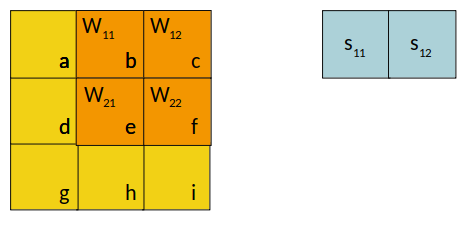
\includegraphics[width=7cm]{figure/conv2d_3.png}}%
\only<5>{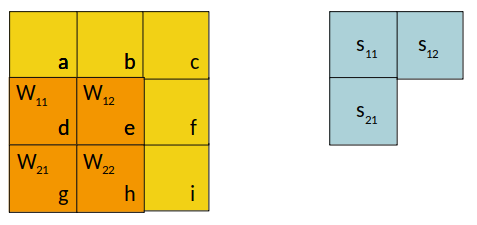
\includegraphics[width=7cm]{figure/conv2d_4.png}}%
\only<6>{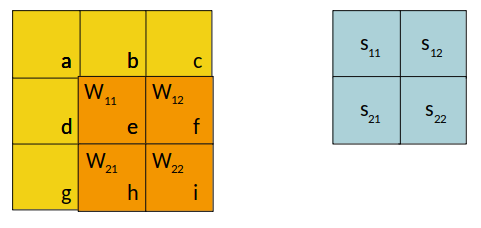
\includegraphics[width=7cm]{figure/conv2d_5.png}}%
\only<7>{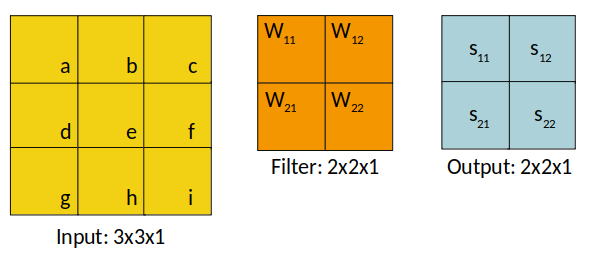
\includegraphics[width=8cm]{figure/conv2d_6.png}}%
\only<8>{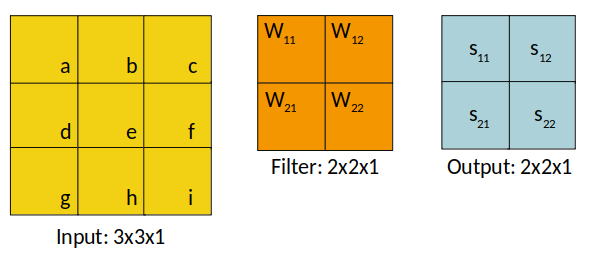
\includegraphics[width=8cm]{figure/conv2d_6.png}}%

\begin{itemize}
\only<1>{\item[] }
\only<2>{\item[] }
\only<3>{\item[] To obtain $s_{11}$ we simply compute the dot product:}
\only<3>{\item[] $s_{11} = a \cdot w_{11} + b \cdot w_{12} + d \cdot w_{21} + e \cdot w_{22}$}
\only<4>{\item[] Same for $s_{12}$:}
\only<4>{\item[] $s_{12} = b \cdot w_{11} + c \cdot w_{12} + e \cdot w_{21} + f \cdot w_{22}$}
\only<5>{\item[] As well as for $s_{21}$:}
\only<5>{\item[] $s_{21} = d \cdot w_{11} + e \cdot w_{12} + g \cdot w_{21} + h \cdot w_{22}$}
\only<6>{\item[] And finally for $s_{22}$:}
\only<6>{\item[] $s_{22} = e \cdot w_{11} + f \cdot w_{12} + h \cdot w_{21} + i \cdot w_{22}$}
\only<7>{\item[] $s_{11} = a \cdot w_{11} + b \cdot w_{12} + d \cdot w_{21} + e \cdot w_{22}$}
\only<7>{\item[] $s_{12} = b \cdot w_{11} + c \cdot w_{12} + e \cdot w_{21} + f \cdot w_{22}$}
\only<7>{\item[] $s_{21} = d \cdot w_{11} + e \cdot w_{12} + g \cdot w_{21} + h \cdot w_{22}$}
\only<7>{\item[] $s_{22} = e \cdot w_{11} + f \cdot w_{12} + h \cdot w_{21} + i \cdot w_{22}$}
\only<8>{\item[] More generally, let $I$ be the matrix representing the input and $W$ be the filter/kernel. Then the entries of the output matrix are defined by $s_{ij} = \sum_{m,n} I_{i+m-1, j+n-1} w_{mn}$ where $m,n$ denote the image size and kernel size respectively.}
\end{itemize}
\end{frame}
%%%%%%%%%%%%%%%%%%%%%%%%%%%%%%%%%%%%%%%%%%%%%%%%%%%%%%%%%%%%%%%%%%

\endlecture
\end{document}
